

\chapter[
ファージMS2を用いた掌付着・洗浄実験の基礎的検討
]{
ファージMS2を用いた掌付着・洗浄\\
\hspace{4.1em}実験の基礎的検討
}

\section{本章の目的}
本章では、指標ウイルスとして大腸菌ファージMS2を用い、
掌表面に付着したウイルスが清浄な水による洗浄で
どの程度除去されるかを基礎的に評価することを目的とした。
第3章で実施した水分付着量測定と同様の動作条件
（浸漬時間、放置時間）でMS2懸濁液に掌を浸漬し、
その後、清浄な水500\,mLを用いて洗浄を行った。
洗浄時に回収された洗浄水中のMS2濃度を
プラーク法により定量し、
洗浄による除去量および残存の傾向を把握する。

本研究は、災害時など水資源が限られる状況を想定しており、
少量の水（本章では500\,mL）で実施可能な
手指洗浄の有効性を定量的に示すことが重要である。
本章で得られる基礎データは、
後続章における洗浄条件の比較検討および
リスク評価（QMRA）に用いる。

%--------------------------------------------------

\section{指標微生物としての大腸菌ファージMS2}
本実験では、大腸菌ファージMS2を指標ウイルスとして用いた。
MS2はヒトに対して非病原性であり、
実験室内で安全に取り扱える点で優れている。
また、粒径が小さく（約25\,nm）、
紫外線照射や塩素消毒などの処理過程における
ウイルス除去・不活性化の評価指標として
国内外で広く使用されている。
さらに、プラーク法により比較的簡便に定量でき、
再現性の高いデータが得られることから、
衛生工学や水処理工学分野において
指標ウイルスとして利用されている。

%--------------------------------------------------
\clearpage
\section{実験材料}
本実験に使用した器具および材料を以下に示す。
\begin{itemize}
  \item MS2ファージ懸濁液
  \item 蒸留水（洗浄用、500\,mL）
  \item 回収用バット（洗浄水回収）
  \item 希釈用器具（チューブ、ピペット等）
  \item プラーク法用培地・宿主菌（大腸菌）および培養器材
\end{itemize}

%--------------------------------------------------

\section{実験方法}

\subsection{浸漬操作および洗浄操作}
実験手順を以下に示す。
\begin{enumerate}
  \item 洗浄用として蒸留水500\,mLを準備する。
  \item MS2懸濁液を30分間攪拌し、濃度を均一化する。
  \item 実験者は事前に手洗い・消毒を行う。
  \item 手の水分を十分に拭き取る。
  \item 掌をMS2懸濁液に5秒間浸漬する。
  \item 浸漬後、20秒間静置し、自然落下する液滴のみを対象とする。
  \item 蒸留水500\,mLを一度に用いて掌を洗浄する。
  \item 洗浄水をバットで回収する。
  \item 回収液を希釈し、プラーク法によりMS2を定量する。
\end{enumerate}

\subsection{測定回数}
測定は被験者5名を対象として実施し、
各被験者について右手および左手を
同一条件下でそれぞれ4回ずつ測定した。
その結果、1名あたり計8回の測定データを取得した。
複数回の繰り返し測定により、
掌の置き方や洗浄操作に伴うばらつきを評価するとともに、
平均値を代表値として用いた。

%--------------------------------------------------

\section{PFU測定および算出方法}
回収した洗浄水は段階希釈後、
プラーク法を用いてMS2のPFU
（Plaque Forming Unit）を測定した。
PFU濃度（PFU/mL）は次式により算出した。

\begin{equation}
\mathrm{PFU/mL} = \frac{N}{V \times D}
\end{equation}

ここで、$N$は観察されたプラーク数、
$V$は接種量（mL）、
$D$は希釈倍率である。

%--------------------------------------------------

\section{残存率の算定方法}
掌表面に付着したファージMS2の洗浄後残存量を評価するため、
本研究では残存率を算定した。
残存率は、掌に初期付着したファージ量に対して、
洗浄後に掌表面へ残存していると推定される
ファージ量の割合を示す指標である。

まず、900\,mL中のMS2ファージ懸濁液の濃度を測定し、
初期ファージ濃度 $C_0$（PFU/mL）を取得した。
次に、第3章で求めた単位面積あたりの水分付着量の平均値
$W$（mL/cm$^2$）と、
該当被験者の掌面積 $A$（cm$^2$）から、
掌に付着した水分量 $V_{\mathrm{hand}}$（mL）を算出した。

\begin{equation}
V_{\mathrm{hand}} = W \times A
\end{equation}

この水分量に初期ファージ濃度を乗じることで、
掌への初期付着ファージ量 $N_0$（PFU）を算定した。

\begin{equation}
N_0 = C_0 \times V_{\mathrm{hand}}
\end{equation}

洗浄後に回収された洗浄水中のファージ濃度を
$C_{\mathrm{rec}}$（PFU/mL）とし、
洗浄水量 $V_{\mathrm{wash}} = 500$\,mL を用いて、
回収ファージ量 $N_{\mathrm{rec}}$（PFU）を次式で算出した。

\begin{equation}
N_{\mathrm{rec}} = C_{\mathrm{rec}} \times V_{\mathrm{wash}}
\end{equation}

以上より、残存率 $R$（\%）は次式により定義した。

\begin{equation}
R = \left(1 - \frac{N_{\mathrm{rec}}}{N_0}\right) \times 100
\end{equation}

本残存率は、掌表面に残存するファージMS2の割合を示し、
洗浄操作による除去効率の評価に用いた。

%--------------------------------------------------
\clearpage
\section{結果・考察}

\begin{figure}[htbp]
  \centering
  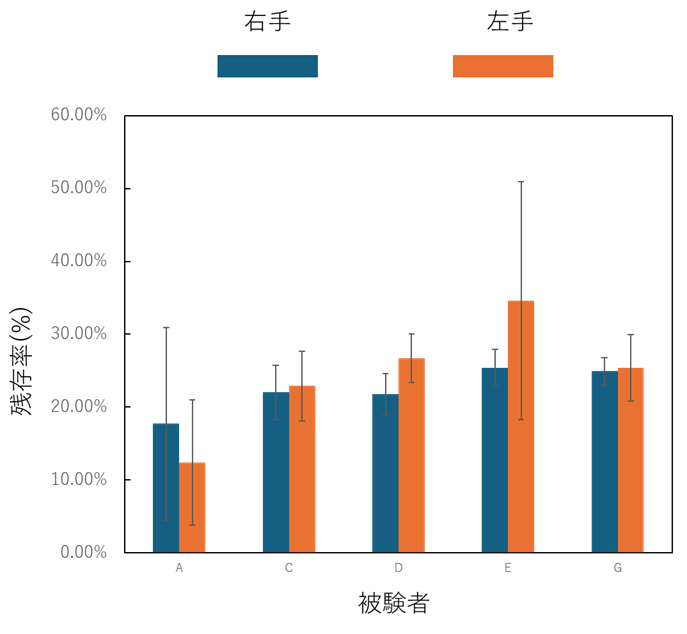
\includegraphics[width=0.85\linewidth]{fig/residual_rate_500ml.png}
  \caption{%
    清浄水500\,mLによる洗浄後の掌へのMS2ファージ残存率\\
    （被験者A，C，D，E，Gにおける右手・左手の平均値および標準偏差）
  }
  \label{fig:residual_rate_500ml}
\end{figure}



清浄な水500\,mLを用いて洗浄を行った結果、
洗浄後の掌へのMS2ファージ残存率は
被験者間でばらつきがみられた。
図\ref{fig:residual_rate_500ml}に、
被験者A、C、D、E、Gにおける
右手および左手の残存率の平均値と標準偏差を示す。

残存率の平均値は、
最小で約12\%、最大で約33\%程度の範囲に分布しており、
同一の水量および操作条件で洗浄を行った場合であっても、
掌表面に残存するMS2量には
被験者ごとの差が生じることが確認された。
このことは、
掌表面の皮膚状態や水分保持特性の違いが、
ファージの残存挙動に影響している可能性を示唆している。

また、右手と左手の残存率を比較すると、
被験者によっては左右で平均値に差がみられた。
一方で、標準偏差が比較的大きい被験者も存在しており、
左右差そのものよりも、
洗浄操作時の水の当たり方や掌の角度、
皮膚表面の微細構造（しわや溝）といった要因が、
残存率のばらつきに寄与している可能性が考えられる。

特に、被験者Eでは残存率の平均値およびばらつきが
他の被験者と比較して大きい傾向を示しており、
同一被験者内であっても測定回ごとの変動が無視できないことが分かる。
この結果は、
単一の測定値のみで洗浄効果を評価することの限界を示しており、
複数回測定による平均値および分布としての評価が重要であることを示唆している。

以上より、
500\,mLという限られた水量による洗浄では、
一定の除去効果は得られるものの、
掌表面には無視できない量のファージが残存することが明らかとなった。
本章で得られた結果は、
後続章において洗浄回数や洗浄方法の違いによる
除去効率を比較検討するための
基礎データとして位置付けられる。


%--------------------------------------------------

\section{本章のまとめ}
本章では、MS2ファージを用いた
基礎的な掌付着・洗浄実験を実施した。
清浄な水500\,mLによる洗浄後にも
一定量のMS2が掌表面に残存することが確認され、
残存率には被験者間でばらつきが認められた。
本結果は、
洗浄条件の違いが除去効率に与える影響を検討する
後続章の基盤となる。
